\documentclass[titlepage]{article}

\usepackage[utf8]{inputenc}
\usepackage[english]{babel} 
\usepackage{lineno, a4wide} % add line numbers
%\linenumbers
\usepackage{setspace} % to use double spacing
\doublespacing

\usepackage{authblk} % author and affiliations
\usepackage{amssymb, amsmath} % for math formulas
\usepackage{amsfonts} % blackboard math symbols
\usepackage[round]{natbib} % citation format
\usepackage{hyperref} % creates links in the document
\usepackage{doi} % Create correct hyperlinks for DOI numbers
\usepackage{times} %Select Adobe Times Roman (or equivalent) as default font

\usepackage{graphicx} % handling figures
\usepackage{subfig} % handling figures
\usepackage[nofiglist,figuresonly]{endfloat} % figures in the end
%\usepackage[nomarkers,figuresonly]{endfloat}
\usepackage{enumitem} % Control layout of itemize, enumerate, description
\usepackage{xcolor} % colored fonts

\usepackage[colorinlistoftodos]{todonotes} % to do comments

\usepackage{subfiles}
\usepackage{parskip}
\usepackage{multirow}
\usepackage[para,online,flushleft]{threeparttable}
\usepackage{rotating}
\usepackage{tikz}
\usepackage{tcolorbox}
\usepackage[export]{adjustbox}[2011/08/13]

\title{
Estimating the cumulative impacts and the zone of influence from multiple anthropogenic infrastructure on biodiversity  \\
{\normalsize in preparation for \textit{Journal of Applied Ecology}}
}

% authors
\author[1,2,*,+]{Bernardo Brandão Niebuhr}
\author[1,*]{Bram Van Moorter} 
\author[1]{Manuela Panzacchi}
\author[3]{Torkild Tveera}
\author[3]{Knut Langeland}
\author[1]{Olav Strand}
\author[4]{Audun Stien}
\author[5]{Per Sandström}
\author[6]{Moudud Alam}
\author[2]{Anna Skarin}

% affiliation
\affil[1]{Norwegian Institute for Nature Research (NINA), Trondheim, Norway}
\affil[2]{Swedish University of Agricultural Sciences (SLU), Uppsala, Sweden}
\affil[3]{Norwegian Institute for Nature Research (NINA), Tromsø, Norway}
\affil[4]{University of Tromsø, Tromsø, Norway}
\affil[5]{Swedish University of Agricultural Sciences (SLU), Umeå, Sweden}
\affil[6]{Dalarna University, School of Information and Engineering/
Statistics, Falun, Sweden}
\affil[*]{Joint first coautorship}
\affil[+]{Corresponding author: Bernardo Brandão Niebuhr, Norwegian Institute for Nature Research (NINA), Trondheim, Norway; bernardo.brandao@nina.no, bernardo\_brandaum@yahoo.com.br}

\date{\today}

\begin{document}

\maketitle

\begin{abstract}

\begin{enumerate}

    \item Most infrastructure and land use change from industrial development take place in landscapes already permeated by multiple human disturbances, leading to cumulative impacts on biodiversity. However, we still lack a comprehensive framework to quantify cumulative impacts. Here we propose an approach to estimate the magnitude and the zone of influence (ZoI) of the impacts of multiple features of an infrastructure and test if their effects accumulate.
    
    \item First, we derive the estimation methods based on either the influence from the nearest feature only or the cumulative influence of multiple features. 
    Second, we perform simulations to distinguish in which scenarios these two measures of influence represent different gradients of spatial variation
    %, and how the area affected by the infrastructure change as the impacts of each of them accumulate. 
    Finally, we illustrate this approach by assessing the cumulative impacts on the space use of mountain reindeer, a species highly sensible to anthropogenic activity and infrastructure. 
    
    \item We present strong evidence of cumulative impacts of private cottages and tourist cabins on reindeer space use, with zones of influence of 10 and 20 km, respectively. This means that considering only the influence of the nearest feature disregards the possibility of cumulative impacts and might limit our understanding of the impacts of landscape change on biodiversity.
    
    \item To make this approach widely accessible for ecologists and analysts dealing with development, wildlife management, and biodiversity conservation, we also provide tools to allow the quantification of cumulative impacts in both R and GRASS GIS through the \verb|oneimpact| R package.
    
    \item \textit{Synthesis and applications}. With our approach we gave a step further in developing a clear way to assess cumulative impacts of infrastructure on biodiversity and ecosystems, with direct application in environmental and strategic impact assessment and integrated land use planning. The approach proposed here allows one to quantify the cumulative impacts of multiple infrastructure of the same type, test if the impacts accumulate, and estimate the zone of influence of multiple types of infrastructure. Even though our examples focus on animal space use, we believe this approach is useful for ecological studies and impact assessments over several fields, from genetics to organisms to populations and communities.
\end{enumerate}

\keywords{\textbf{Key-words:} (up to 8) cumulative effects, Anthropocene, habitat fragmentation, habitat loss, \textit{Rangifer tarandus}, density, nearest neighbor distance, scale of effect, kernel filter, distance-weighting}

\end{abstract}

\section{Introduction}

Human-induced land cover modifications and infrastructure from industrial development are spread and increasing at an accelerated pace across all regions of the world \citep{venter_sixteen_2016,ibisch_global_2016}, including all global biodiversity hotspots \citep{sloan_remaining_2014}, and are among the main causes of biodiversity declines \citep{benitez-lopez_impacts_2010,newbold_global_2015}. Most new landscape changes take place not in intact habitats but in landscapes already permeated by multiple disturbances to wildlife  \citep{barber_roads_2014,kowe_quantitative_2020}. As a consequence, the effects of such new modifications might accumulate and interact in complex ways with the preexisting anthropogenic stressors, potentially leading to synergistic, interactive, or unpredictable outcomes, different from those of each separate source of disturbance \citep{naugle_unifying_2011}. This process is tackled in the discussion about ``nibbling" and ``piece-meal development" \citep{nellemann_progressive_2003} and have been addressed under the name of cumulative anthropogenic impacts \citep[Box 1; ][]{gillingham_integration_2016}. Indeed, cumulative impacts are a central issue in ecological studies and environmental impact assessments and a priority for making effective, knowledge-based decisions on land use planning, designing mitigation actions, and avoiding higher impacts of industrial development on ecosystems \citep{krausman_cumulative_2011, laurance_roads_2017}. There have been increasing efforts to better define, review, and outline approaches for cumulative impact assessment \citep{naugle_unifying_2011,gillingham_integration_2016}, yet we still lack a comprehensive framework to quantify cumulative impacts and thus concretely help sustainable land use planning.

Anthropogenic infrastructure have direct consequences in the area where they are built (e.g. road kills and habitat modification from road building), but they might also indirectly affect species and ecological processes up to several kilometers from the infrastructure locations \citep{johnson_cumulative_2005,torres_assessing_2016}, e.g. by creating avoidance and reducing the probability of animal occurrence \citep{trombulak_review_2000,harris_grappling_2011}. Therefore, two key factors to be assessed in cumulative impact studies are the magnitude of the impact from infrastructure and the scale or area where this impact is present \citep[Box 1; ][]{naugle_unifying_2011}. Understanding the \textit{effect size} or \textit{magnitude of the impact} is generally the core of most research focused on impacts and is tackled by estimating which factors influence focal organisms and processes and how strongly they are affected, generally through a combination of biological and environmental data and statistical modeling [Box 1; REF]. The spatiotemporal \textit{scale} or \textit{zone} of influence (ZoI) is intrinsically related to the magnitude of the impacts and corresponds to the area (and sometimes the period) within which there are detectable impacts from different landscape modifications on the process of interest, but is commonly expressed in terms of distances --- the distance from or radius around the disturbance sources which defines the affected area \citep[Box 1; ][]{polfus_identifying_2011, boulanger_estimating_2012}. Most environmental impact assessment studies still focus on single projects at small spatiotemporal scales, and even ecological studies conducted at larger extents hardly account explicitly for cumulative effects of multiple infrastructure at multiple scales, when estimating the magnitude and ZoI of anthropogenic effects on biodiversity \citep{johnson_regulating_2011, mcgarigal_multi-scale_2016}. 

%The term ``scale" has been used in multiple contexts in ecology (e.g. scale as landscape grain and extent; spatial and temporal scales and the scale of ecological organization; \citealt{wiens_spatial_1989}; scale or level of animal habitat selection; \citealt{lima_towards_1996}) and has led to important advances in ecological theory \citep{fahrig_effects_2003, mcgarigal_multi-scale_2016}. However, to avoid misunderstandings with the nomenclature, here we use the term Zone of Influence (ZoI) to refer to the area or distance from infrastructure where there is any effect on biodiversity \citep{naugle_unifying_2011}.

Infrastructure and disturbance impacts can accumulate at least over time and space, as a result of the sum or interaction of the impacts of different types of infrastructure or multiple features of same-type infrastructure \citep{wolfe_response_2000}. The consequences of multiple types of infrastructure are generally included in ecological models by careful evaluation of their correlations \citep{dormann_collinearity_2013} and subsequently through the inclusion of additive or interactive terms in statistical model specification, to control for their mutual potential influence on the studied system [REF]. This allows one to estimate the coefficients that represent the magnitude of the impact for each infrastructure or their combination. Alternatively, other studies combine multiple disturbances in a single measure of cumulative effect before fitting statistical models \citep{polfus_identifying_2011, venter_sixteen_2016, tucker_moving_2018}. As for the influence of multiple infrastructure of the same type, most commonly they are either considered by changing the variable's level of spatial organization (e.g. urban areas or wind parks instead of a combination of buildings and turbines, respectively) or ignored by considering only the effect of the nearest infrastructure feature \citep[e.g.][]{torres_assessing_2016}. 

The determination of the ZoI for multiple infrastructure is intrinsically related to the magnitude of the impacts, even though it is not always present on impact studies, maybe because of the challanges involved in the task  \citep{quinonezpinon_design_2007}. When estimating the ZoI, the concept of ecological threshold \citep{huggett_concept_2005} and analytical procedures developed therein are commonly used \citep{ficetola_ecological_2009}. Under this framework, the estimation of the zones of influence is often carried out by fitting piece-wise regression or other non-linear regression models \citep[such as an exponential decay or generalized additive models;][]{skarin_out_2018, ficetola_ecological_2009} to the measured response of an ecosystem to an infrastructure as a function of distance. This distance is typically the distance to the nearest instance of this infrastructure type, ignoring potential additive or cumulative effects of multiple instances or features of an infrastructure \citep[e.g ][Box 1]{torres_assessing_2016}. Besides, this approach is generally limited to the assessment of thresholds for only one or a few types of infrastructure \citep[e.g.][]{boulanger_estimating_2012}, since its computation requires repeated fitting and might become impracticable for a large number of factors \citep{lee_estimating_2020}. 

Another approach to estimate the ZoI may be found under the umbrella of the discussion about spatial and temporal \textit{scales of effect}, common in the evaluation of species-landscape relationships. In this context, the number of features is averaged for multiple spatial extents surrounding focal study sites \citep{jackson_are_2015} or filtered (\textbf{weighted?}) using neighborhood analysis over several different extents or radii (generally termed ``scales"), creating a series of infrastructure density maps \citep{mcgarigal_multi-scale_2016}. These spatial scales are generally linked to the spatial and temporal dimensions of the infrastructure considered, as well as to the expected temporal scale of the biological response to such infrastructure. Each of these maps is tested against the ecological response variables to assess the extent where the impact is stronger, either \textit{a priori} to select biologically meaningful scales, based on R\textsuperscript{2}, information criteria such as AIC or BIC, or other measures of model performance and explanatory power \citep{jackson_are_2015, huais_multifit_2018}, or \textit{a posteriori} (after model fitting) \citep{thompson_influence_2002}. This approach characterizes what is called multi-scale analyses \citep[e.g.][]{zeller_multi-level_2017}, in contrast to single-scale analyses in which the effect of all variables is evaluated with the same extent. Multi-scale analyses brought important advances for landscape and environmental impact studies \citep[e.g.][]{mcgarigal_multi-scale_2016}, even though in many of them the scale of effect was not properly evaluated \citep{jackson_are_2015}. However, the key here is that these approaches have hardly been put into the framework of cumulative impact assessment \citep[but see, for instance,][]{polfus_identifying_2011}. 
\todo[inline]{I need to review this paragraphs later to make sure the idea of ``scale" is not confusing. Maybe replace by more precise terms, when possible.}

Building upon this literature, we propose an approach to estimate the magnitude and the ZoI of the impacts of multiple features of an infrastructure and test if they accumulate. First, we derive the estimation methods based on either the influence from the nearest feature only or the cumulative influence of multiple features (Box 1, Fig. \ref{fig:zoi_conceptual}), using habitat selection analyses as an example. Second, we perform simulations to distinguish in which scenarios these two measures of influence represent similar or different spatial gradients, to understand how the spatial configuration of landscape modification might lead to higher expected cumulative impacts. 
%We also estimate how the area affected (Box 1) increases as the impacts of multiple infrastructure accumulate over these different scenarios. 
Finally, we illustrate our approach by assessing the cumulative effects on the space use of the tundra's flagship species, the mountain reindeer (\textit{Rangifer tarandus tarandus}). We also provide tools to allow an easy implementation of the cumulative approach presented here in R \citep{r_core_team_r_2020} and GRASS GIS \citep{grass_development_team_geographic_2017} through the \verb|oneimpact| R package. Even though our examples focus on animal space use, we believe this approach is relevant for ecological studies and impact assessments over several fields, from genetics to organisms to populations and communities.

\begin{tcolorbox}[width=1.3\textwidth,center,colback=yellow!5,colframe=yellow!75!black,title={Box 1 -- Definitions}]

\begin{description}

    \item[Cumulative impacts] The term \textbf{impact} is used here to represent the consequences of human-made changes on ecological response variables, such as measures of biodiversity or ecological processes \citep{naugle_unifying_2011}. Thus, impacts represent the functional responses of species and processes to human activity. In this context, \textbf{cumulative impacts} are a result of the interaction between the the effects of different infrastructure (e.g. houses, turbines, roads, dams) and depend on the number of features of an infrastructure, their spatial distribution, and co-occurrence with other infrastructures, and might differ for distinct species, values, or processes - possibly leading to stronger negative impacts for some, if compared to the impact of a single infrastructure, or even to benefits for others.
    
    \item[Impact dimensions] Here we analytically decompose the impacts into their \textbf{magnitude} and the \textbf{influence function} that defines how far from the disturbance source the impact reaches. A given infrastructure (e.g. tourist cabin) might affect a certain process (e.g. an species occurrence) strongly or weakly (magnitude), and this impact might decrease fast or extend over several kilometers (influence function).
    
    \item[Magnitude of the impact] The magnitude of the impact describes how strong is the effect pf a variable over a given biological response, and is described here by the model coefficients ($\beta$'s in eq. \ref{eqn:HSF}). 
    
    \item[Influence] The term \textbf{influence} is used here in a pragmatic way and represents the function $\phi$ that sets how the impacts of an infrastructure feature change with the distance to such feature, and is the basis for defining the zone of influence
    %and area affected by the infrastructure, for a given biological response. 
    The influence of a feature might follow different \textbf{influence functions} (also called weighting functions, smoothing filters, or decay functions). It can be constant up to a given threshold distance or decrease in different ways with increasing distance from it (Fig. \ref{fig:zoi_conceptual}A). When multiple features of an infrastructure are present, one can assume that either only the nearest features influence the response (eq. \ref{eqn:HSFnearest}) or that the influence of multiple features accumulate (eq. \ref{eqn:HSFcuminf}, Fig. \ref{fig:zoi_conceptual}B).
    
    \item[Zone of Influence] The \textbf{zone of influence} or \textbf{ZoI} is the maximum distance from an infrastructure feature where it influences or affects a given biological response. For non-vanishing functions (e.g. exponential, Gaussian), a threshold must be set to define the ZoI -- e.g. the distance at which the influence function goes below 0.05 or 0.01. 
    %Here we call this threshold $\phi_{limit}$.
    In the landscape ecology literature the ZoI is often called the \textit{scale of effect} of a given covariate in space \citep[e.g.][]{jackson_are_2015}; we use the term ZoI to avoid misunderstandings derived from the different definitions of \textit{scale}. 
    
    %\item[Affected area] Once the influence function and the ZoI for a type of infrastructure and a biological response are found, one can estimate the area affected or under influence of the infrastructure. When only the nearest feature influences the process of interest, the area affected is directly calculated from the influence function. When the influence of the features accumulate, and as the number of features increase, the area affected might also increase.

\end{description}
\end{tcolorbox}

\section{Deriving the estimation of the cumulative influence of multiple features}

We first derive the cumulative influence of multiple features of an infrastructure type, e.g.\ roads, houses or tourist resorts, on space use. To illustrate it, we use as an example a habitat selection analysis, which aim at discriminating what sets of environmental conditions are selected or avoided by animals, based on ecological data such as species occurrence or movement data and use-availability designs \citep{johnson_resource_2006,fieberg_how_2021}. The main element in habitat selection approaches is the habitat selection function (HSF) $w(\textbf{X})$, a function proportional to the probability of selection of a given space resource unit, depending on the frequency of used and available resource units \citep{thurfjell_applications_2014}. The HSF $w(\textbf{X})$ is function of a vector of predictor variables $\textbf{X} = X_1,X_2, ...,  X_k$, which here correspond to $k$ different types of infrastructure, but might also represent other landscape modifications or spatiotemporal variables. In its parametric form, the HSF might be represented by

\begin{equation}
\centering
\label{eqn:HSF}
    w(\textbf{X}) = \exp \left( \beta_0 + \overbrace{\beta_1 X_1}^\text{A) Infrastructure type 1} + \overbrace{\beta_2 X_2}^\text{B) Infrastructure type 2} + \underbrace{\beta_{12} X_1 X_2}_\text{D) Interaction infrastructure types 1 and 2} + ... + \overbrace{\beta_k X_k}^\text{C) Infrastructure type k} \right)
\end{equation}

where $\beta_k$ represents the magnitude of the impact (coefficient or effect size) of the infrastructure of type $k$. In its simplest form, here \textit{the cumulative impact of different types of infrastructure} is given by the additive effects of the $k$ infrastructure types (e.g. terms A, B, and C in equation \ref{eqn:HSF}) and possibly by interaction terms between variables (such as term D in equation \ref{eqn:HSF}, with an interaction coefficient $\beta_{12}$), that allow for non-linear, joint effects caused by the co-occurrence of different types of infrastructure. 

To derive the cumulative impact of multiple infrastructure of the same type, we start by defining verbally two representations of the spatial influence of infrastructure: the influence of the nearest feature alone and the cumulative influence of multiple features (Box 1, Fig. \ref{fig:zoi_conceptual}). Note that we refer to the term ``influence" instead of ``distance", since we are generally referring to decay functions that decrease towards zero as the Euclidean distance from the infrastructure increases, and possibly vanish at a given point (the zone of influence).

First, within the ZoI, the influence of an infrastructure feature (e.g. a house or road) might follow different functions -- it can be either constant (threshold curve, Fig. \ref{fig:zoi_conceptual}A) or decrease as one moves away from the infrastructure (e.g. linear and Gaussian curves, Fig. \ref{fig:zoi_conceptual}A). 
Whether the influence of a given infrastructure follows one of these or other functions is to be determined empirically \citep{miguet_how_2017}. The simplest assumption, widely used in the literature, is that all the area within the ZoI is affected equally \citep[e.g][]{quinonezpinon_design_2007}, even though it might be more reasonable to consider that the influence is higher close to the infrastructure \citep[][]{skarin_out_2018, zeller_multi-level_2017}. Second, the effect of the infrastructure might depend either on the nearest infrastructure alone or on the cumulative influence of several infrastructure (Fig. \ref{fig:zoi_conceptual}B). In the former case, the influence is similar when one approaches a single, isolated house or a small village, for example. In the latter, the influence of nearby houses accumulate and might be greater than that of a single, isolated house.

\begin{figure}[h]
\centering
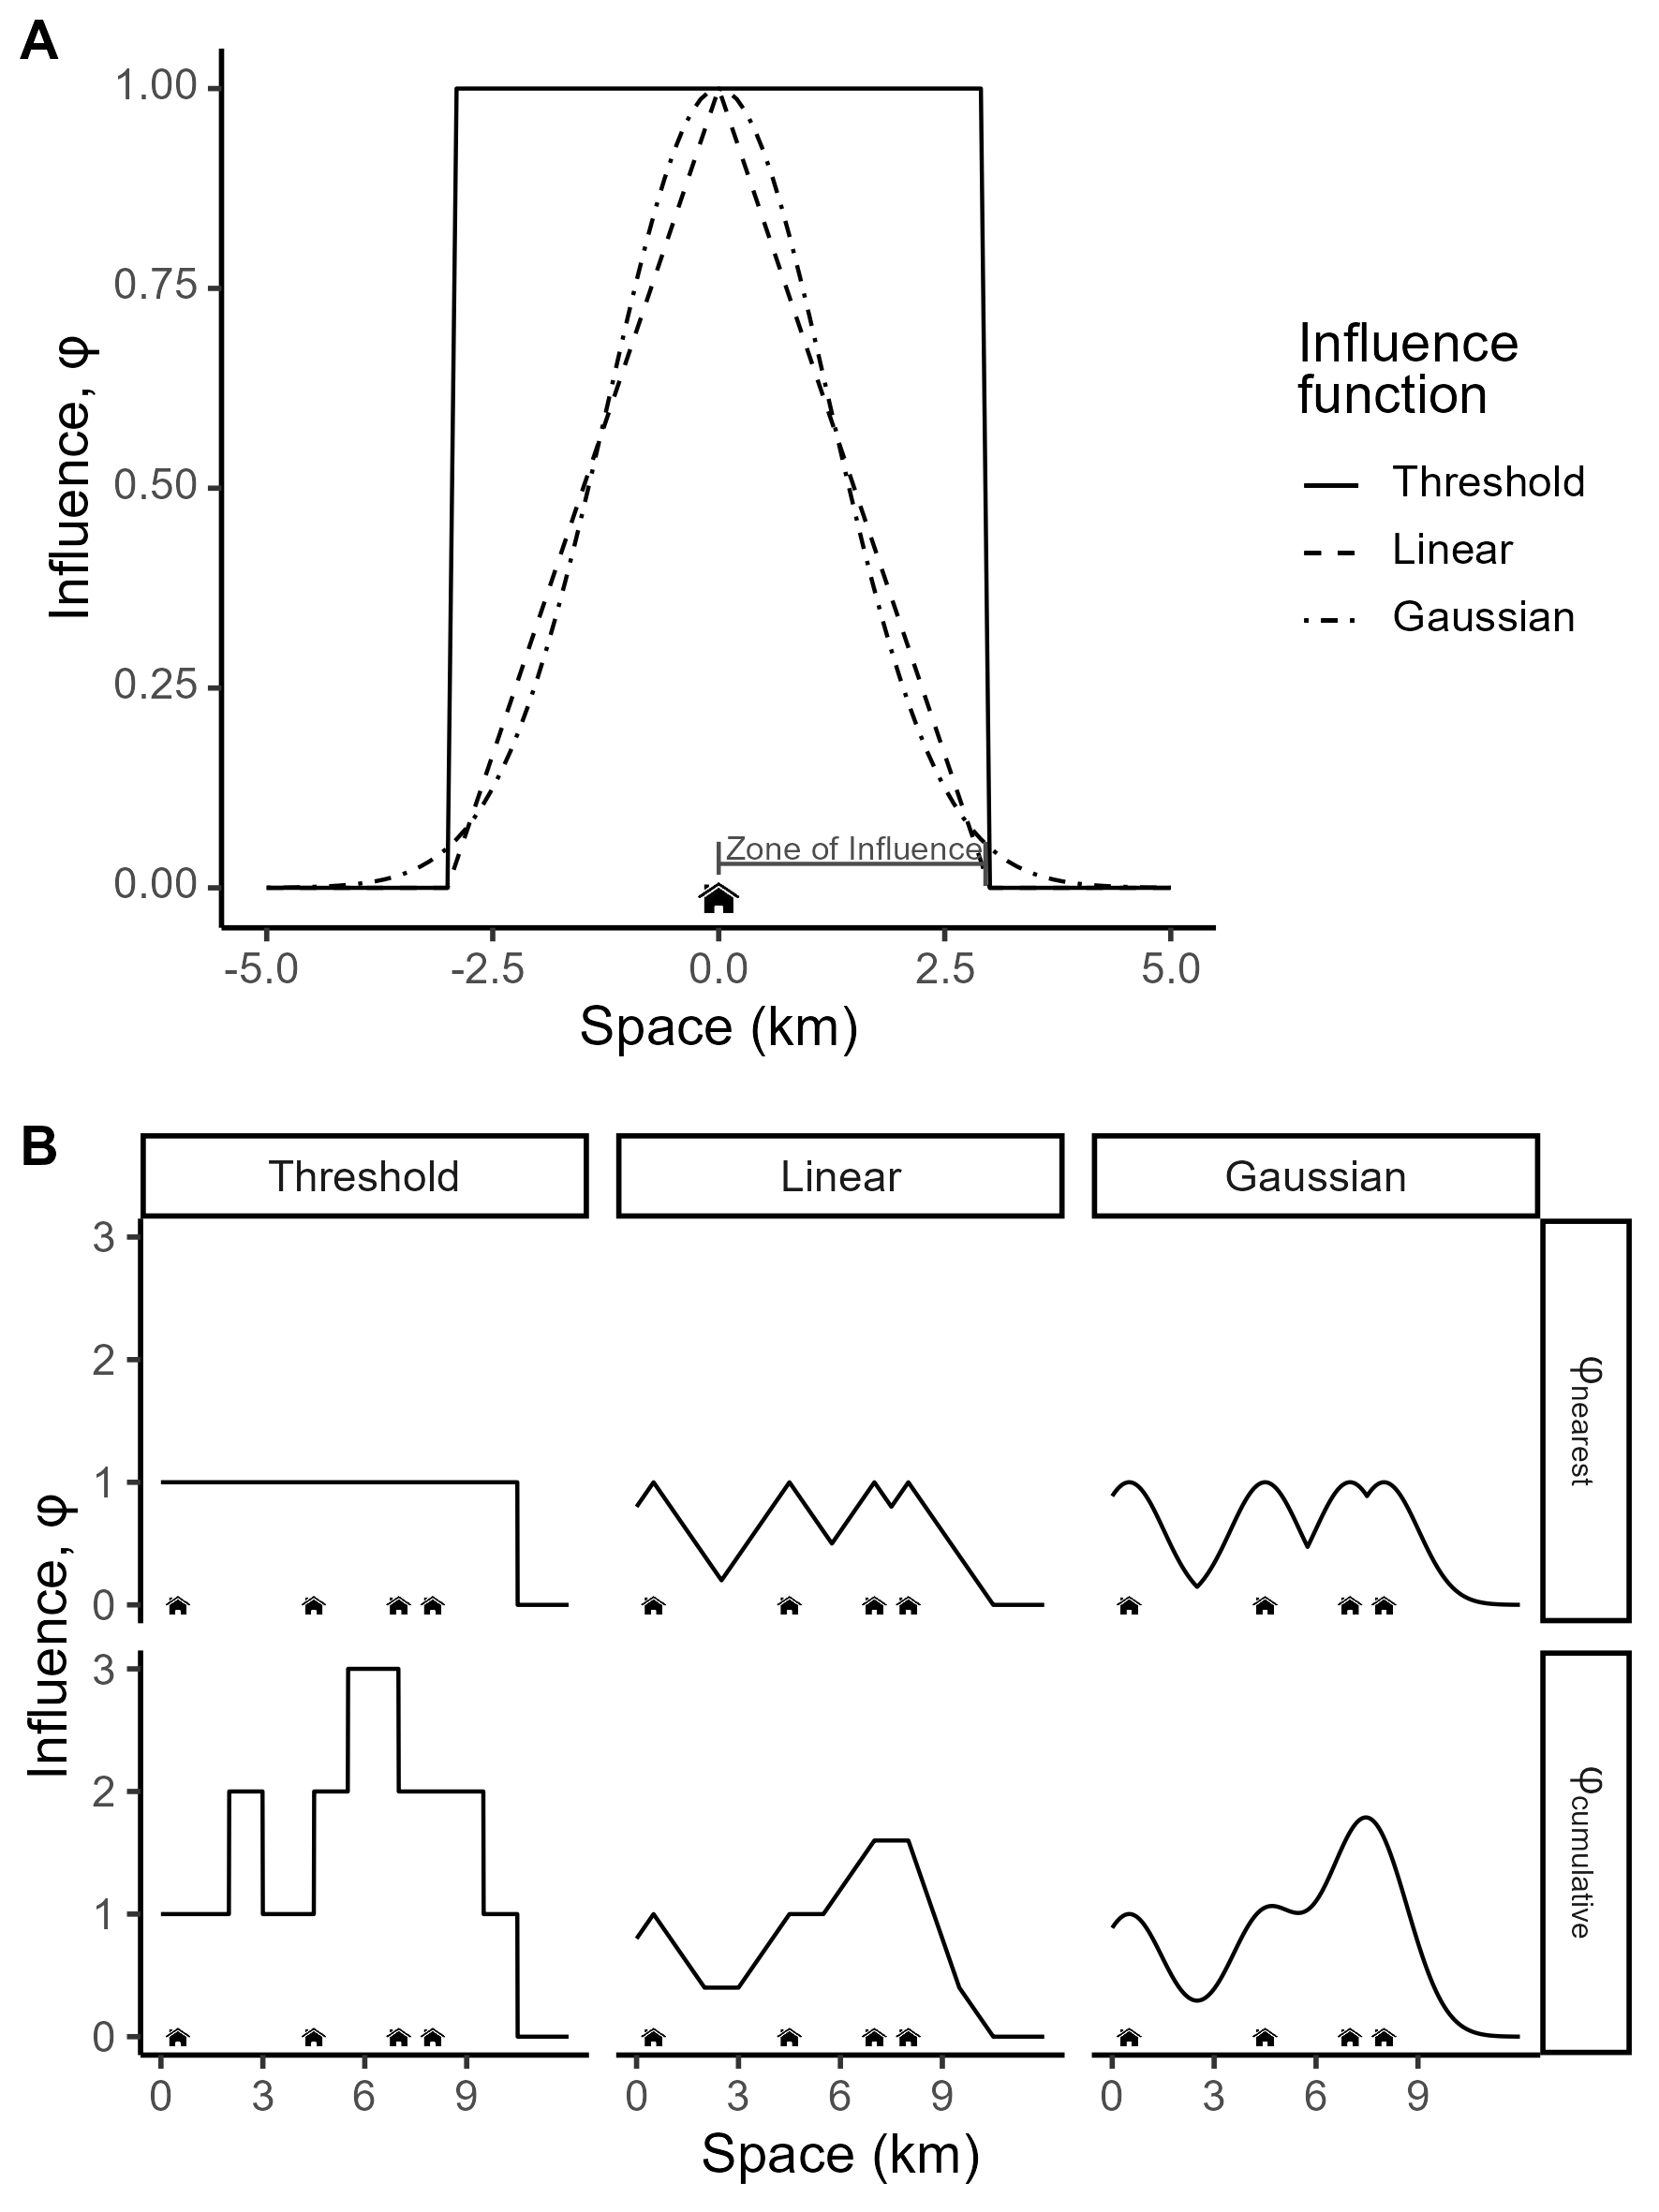
\includegraphics[width=0.9\textwidth]{figures/ZoI_conceptual.png}
\caption{\label{fig:zoi_conceptual} Illustration of the influence ($\phi_{i_k}$) of infrastructure features against the distance from those features ($d_{i_k}$), simplified for one dimension and using houses as an example. (A) Examples of influence functions according which the influence of the house might vary. A house has only an influence within its zone of influence (here $ZoI_{i_k} = 3 \text{ km}$). For the threshold function, the influence remains constant within the ZoI and drops to zero beyond it, whereas for both the linear and Gaussian functions it declines monotonically within the ZoI. For functions that asymptotically approach zero, a cutoff must be selected to characterize the ZoI (here the ZoI is the distance where the influence decreases to $\phi_{i_k} < 0.05$). (B) Representation of the influence of multiple houses by considering only the nearest feature (upper row) or the cumulative influence of multiple features (bottom row), for different influence functions. If only the nearest house affects space use, the influence will not go above one; when all houses act cumulatively, their cumulative effect can be much higher than one.}
\end{figure}

To translate those representations into a mathematical form, now we decompose each of the linear terms (i.e. A, B, C, ...), in equation \ref{eqn:HSF}. Suppose that in the landscape there are $n_k$ features of the same type of infrastructure $k$, and let the influence of the feature $i$ of an infrastructure \textit{k} follow an influence function \citep[or ``weighting function", ][]{miguet_how_2017} $\phi_{i_k} = f(d_{i_k}; ZoI_k)$, where $d_{i_k}$ is the distance to a feature ($i_k$) of infrastructure type $k$ and $ZoI_k$ is its zone of influence. Figure \ref{fig:zoi_conceptual}A shows a few possible shapes for the function $\phi_{i_k}$. We can sum the effect of each feature on animal space use, so that the linear terms in equation \ref{eqn:HSF} become:

\begin{equation}
\label{eqn:HSFterm}
    \beta_k X_k = \sum_{i=1}^{n_k} \beta_{i_k} \phi_{i_k}
\end{equation}

Typically, only the nearest feature is considered, resulting on the implicit assumption that $\beta_i = 0$ for all $i > 1$ (where the features are ordered by increasing distance). Thus, eq. \ref{eqn:HSFterm} turns into:

\begin{equation}
\label{eqn:HSFnearest}
\begin{split}
    \beta_k X_k & = \beta_{1_k} \phi_{1_k} \\
                & = \beta_{1_k} \phi_{nearest_k}
\end{split}                
\end{equation}

where $\phi_{nearest_k}$ is the influence of the nearest feature ($i = 1$) of the infrastructure type $k$ (see Fig. \ref{fig:zoi_conceptual}B). However, possibly a more reasonable assumption would be that $\beta_{i_k} = \beta_{{(i+1)}_k} = \beta_{{(i+2)}_k} = ... = \beta_k$, i.e. that all features of a given type present the same influence around them and all $\beta$'s are identical. Thus, eq. \ref{eqn:HSFterm} is reduced to:

\begin{equation}
\label{eqn:HSFcuminf}
\begin{split}
    \beta_k X_k & = \beta_k \sum_{i=1}^{n_k} \phi_{i_k} \\
                & = \beta_k \phi_{cum_k}
\end{split}
\end{equation}

where $\phi_{cum_k} = \sum_{i=1}^{n_k} \phi_{i_k}$ is the cumulative influence measure and is a proxy to 
%what has been called 
the ``density" of features in space \citep[e.g.][]{panzacchi_searching_2015}. The cumulative influence measure might be easily calculated using geographical information systems, e.g. through neighborhood analysis, and can be rescaled to meaningful measurement scales, such as the number of point features per km\textsuperscript{2} or the length (in km) of linear infrastructure per km\textsuperscript{2}. Equation \ref{eqn:HSFcuminf} presents the simplest possibility of considering the cumulative effect of features of the same type. For the derivation of similar equations for variables represented as lines and areas, see Appendix A.

Analogous to \citet{lee_estimating_2020}'s recasting of the identification of the ZoI of a single (i.e. the nearest) infrastructure as a model selection rather than a parameterization problem, with this definition we can also estimate the cumulative effect size and the ZoI of features using model selection, which allows the process to be performed for different types of infrastructure. Beyond that, this formulation makes it possible to test for the presence of cumulative impacts of anthropogenic landscape changes by comparing models with either of the two influence measures (eq. \ref{eqn:HSFnearest} and \ref{eqn:HSFcuminf}), both based on the same decay function.

%Finally, we can move beyond the identification of the distance under influence around infrastructure (the ZoI) and define the area affected, which is the area within the ZoI of all infrastructure in the landscape combined (Box 1). For this purpose, we define a $\phi_{limit}$, the threshold above which we consider there is impact of infrastructure -- the same used to define the ZoI for non-vanishing function (e.g. Gaussian). Given this, the area affect $A_k$ by all infrastructure of type $k$ in a landscape is given by:

%\begin{equation}
%\label{eqn:area_affected}
%    A_k = \iint_\Omega \Phi_{k}(x,y) \,dx\,dy
%\end{equation}

%where 

%\begin{equation}
%\label{eqn:area_affected2}
%\begin{split}
%    \Phi_k = \begin{cases}
%    1 & \text{if $\phi_k >\phi_{limit}$} \\
%    0 & \text{otherwise}
%    \end{cases}
%\end{split}
%\end{equation}

%and $\Omega$ is the area of the whole landscape. Here we use $\phi_{limit} = 0.05$. As we show in the next section, the area affected depends on whether a landscape presents a few or many features of an infrastructure and on their spatial distribution, as well as on whether the influence of the nearest feature or the cumulative influence are considered.

\section{When do the influence of the nearest feature and the cumulative influence diverge?}

Whether the spatial variation represented by the cumulative influence of multiple features of an infrastructure is similar or not to the influence of the nearest feature depends on the spatial distribution of the infrastructure as well as its zone of influence. To illustrate when they converge and diverge, we simulated $30 \times 30$ km landscapes with a constant number of point features (e.g. houses, cabins, turbines; $n = 100$) distributed following different spatial patterns, in a gradient of clustering, from regular and random to clustered (Fig. \ref{fig:simulated_landscapes}; Appendix B). For each scenario we calculated the two measures of influence (nearest feature, $\phi_{nearest}$, and cumulative, $\phi_{cum}$) for a range of values of ZoI (from 20 m to 12 km), using a linear decay function \citep[Fig. \ref{fig:zoi_conceptual}; ``Bartlett" or tent-shaped decay;][]{harris_use_1978}, for which the ZoI is easily defined as the distance at which the function decreases to zero. We then compared the resulting influence spatial patterns through Pearson correlation of the values of the two measures at the same coordinates (see details in the Appendix B). 

\begin{figure}[h]
\centering
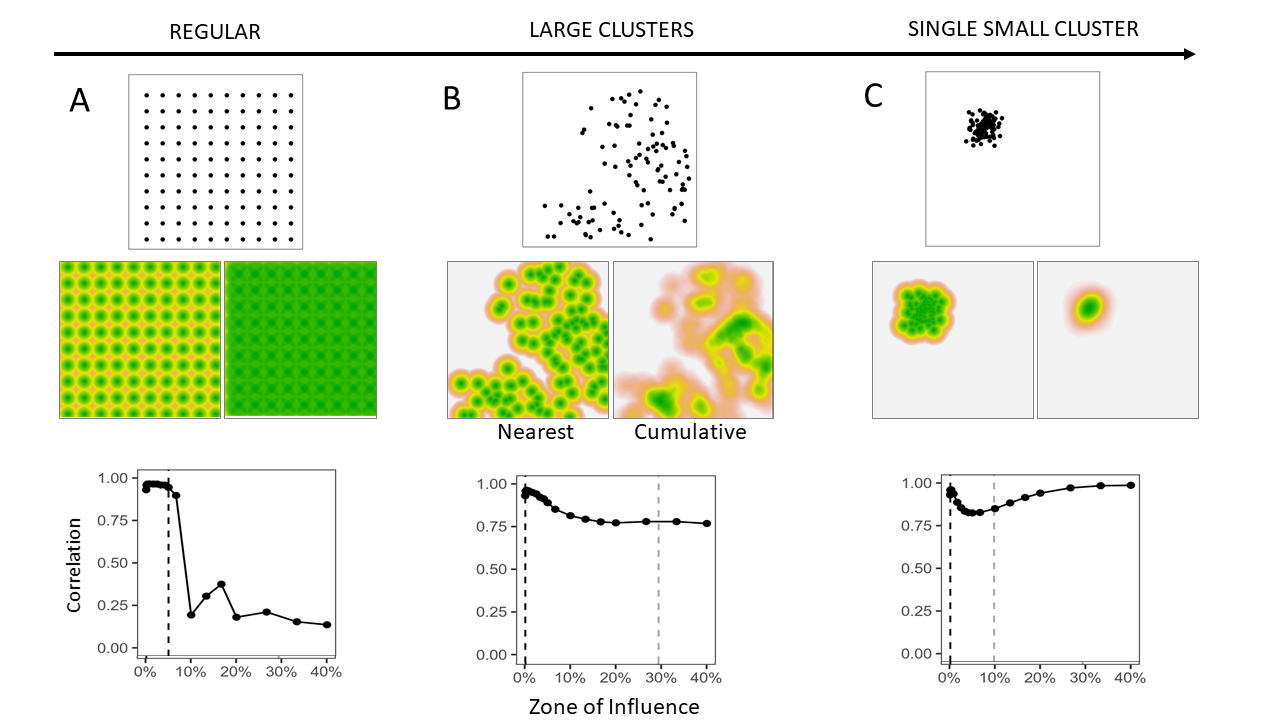
\includegraphics[width=1.3\textwidth,center]{figures/simulated_landscapes.png}
\caption{\label{fig:simulated_landscapes} Representation of the influence of nearest feature ($\phi_{nearest}$) and the cumulative influence ($\phi_{cum}$) in landscapes with point infrastructure spatially distributed in a gradient of clustering, from (A) a regular distribution (e.g. a large solar power plant in a flat area) to (B) a set of clusters (e.g. a wind industrial area formed by wind turbines built in the mountain tops) to (C) only one cluster (e.g. isolated village or urban center). The central panel shows  a visual comparison between the influence of the nearest feature (left) and the cumulative influence (right) between simulated landscapes following each of those patterns when $ZoI = 0.1 \cdot \text{landscape extent}$ (higher than the average distance between infrastructure features, see Appendix B). The lower panel shows the correlation between the influence of the nearest feature and cumulative influence in each scenario, as their ZoI increases. The dashed vertical lines show half the the minimum distance between features (black), beyond which there are cumulative effects of the different infrastructure, and the size of the feature clusters (grey), beyond which the correlation stops decreasing.}
\end{figure}

%The correlation between the influence measures was generally higher for clumped distribution of features than for regularly or randomly distributed points. 
When $ZoI/2$ is smaller than minimum distance between features, both measures of influence are similar and their correlation is maximum (Fig. \ref{fig:simulated_landscapes}; $\text{correlation} = 1$ for all ZoI values below the black dashed vertical line). This happens because the ZoI of each feature is not large enough to interact with each other. As the ZoI increases, the effect of nearby features starts to sum and the two measures of influence begin to represent different patterns of spatial variation. This is valid for scenarios with random, regular, and slightly clustered distributions of infrastructure features (Fig. \ref{fig:simulated_landscapes}A,B, Fig BXX in Appendix B). In contrast, as the distribution of features gets more clumped and distributed in smaller clusters (up to a limit with a single small cluster, Fig. \ref{fig:simulated_landscapes}C), the correlation between the influence measures goes through a point of inflection as the ZoI increases, beyond which it increases with ZoI (Fig. BYY in Appendix B). The point where the correlation between the influence measures stop decreasing is defined by the size of the clusters (grey dashed vertical line in Figs. \ref{fig:simulated_landscapes}B,C). For ZoI values larger than the cluster size, the two influence measures start to converge again. That is the point beyond which it might get harder to distinguish between the effect of each feature alone, regardless of the influence measure, and the effect of a collection of features transforms into that of a ``super-feature" (e.g. a group of houses or wind turbines behave as an urban area or a wind park, respectively). 
Overall, the correlation between the influence measures was high between scenarios. In some empirical cases it might be difficult to distinguish whether the impacts of a given infrastructure type accumulate or not. However, in other cases (such as the correlation inflection point mentioned above) it might be easier to detect differences and test for cumulative effects.

% Since a great part of the literature uses as measure of infrastructure influence transformations of the Euclidean distance from the nearest feature, such as the logarithm or the scales distance, we also calculated the logarithm of the Euclidean distance to the nearest feature to compare with the cumulative influence.

 %Here we simulated landscapes with point infrastructure because of the simplicity to represent them and place them following different patterns. We believe these simple cases might also provide insights on when $\phi_{nearest}$ and $\phi_{cum}$ are similar for other types of infrastructure, for instance linear infrastructure (e.g. roads, railways, and power lines) and higher dimensional landscape changes defined by polygons and areas (e.g. dams, mining or forestry areas, and deforestation sites). However, we recognize that those patterns can get more complex as these structures and spatial patterns extend over large distances and areas, and a further assessment of when these influence measures converge might be needed. \todo{better to place this paragraph in the discussion?}

\section{Empirical demonstration: cumulative influence of infrastructure on reindeer space use}

\subsection{Study area, ecological data, and methods}

In our empirical demonstration we aimed to assess if and how the impacts of multiple infrastructure affect mountain reindeer space use during summer in Southern Norway. Wild reindeer are highly sensible to human activity, and the populations in Norway are the last remaining ones of this species in Europe. We used GPS tracking data from the Hardangervidda reindeer population, the largest population of wild mountain reindeer (Fig. \ref{fig:prediction_maps}). During summer, the area is mostly used for tourism. It has 14,154 private cottages, 26 large tourist cabins, and hundreds of kilometers of trails, besides roads and small tourist cabins (Fig. C2). We used data from 48 (??) female reindeer collected between 2001 and 2010 \citep[see][for further details]{panzacchi_searching_2015} and selected July as a month representative of the summer. To assess reindeer habitat selection using a use-availability setup, each used GPS point was compared against 9 available locations created at random within the area occupied by the population (Fig. \ref{fig:prediction_maps}) and annotated with environmental covariates.

To account for bio-climatic-geographical variation in environmental characteristics we used the four first components from a large principal component (PC) analysis conducted for Norway \citep{bakkestuen_step-less_2008}, which correspond to gradients of (1) PC1 - continentality, (2) PC2 - altitude, (3) PC3 - terrain ruggedness, and (4) PC4 - solar radiation. We included a quadratic term for PC1 and PC2 to account for non-linear responses \citep{panzacchi_searching_2015}. We also used the NORUT land cover map with 25 vegetation classes, which we further grouped \citep[see Table C2][]{johansen_vegetasjonskart_2009}. Because of correlations among covariates, and to keep model fitting relatively simple, we included two anthropogenic variables: private cottages and large tourist cabins, for which we estimated the cumulative impacts.

For each infrastructure type we calculated the influence measures for 8 different ZoI: 100, 250, 500, 1000, 2500, 5000, 10000, and 20000 m. For each ZoI, we used four influence functions, to account for different shapes of the variation of the infrastructure influence within the ZoI (Fig.~\ref{fig:zoi_conceptual}A): threshold, linear decay, Gaussian decay, and exponential decay, and made two assumptions for the impact of additional features, leading to the measures of influence from the nearest feature ($\phi_{nearest}$, eq. \ref{eqn:HSFnearest}) and cumulative influence ($\phi_{cum}$, eq. \ref{eqn:HSFcuminf}; see Fig.~\ref{fig:zoi_conceptual}B). We then fitted HSFs (eq. \ref{eqn:HSF}) combining the effects of infrastructure, land cover, and bio-climatic data using the function \verb|coxph| from the \verb|survival| package in R \citep{therneau_package_2020, therneau_modeling_2000}. 

Model fitting consisted in two steps. We first fitted single-infrastructure models in a procedure of variable selection \citep{burnham_model_2002} to assess the most likely influence functions and ZoI for each infrastructure type, while checking for the correlation between covariates. Single-infrastructure HSF were fitted using the \verb|multifit| function in R \citep{huais_multifit_2018} and compared using AIC. Second, using the most likely influence functions and ZoI from the single-infrastructure models, we fitted multi-infrastructure HSF to assess the combined impacts of multiple types of infrastructure, in an approach similar to LaForge et al. \citealt{laforge_process-focussed_2015}. 

To quantify the impacts of infrastructure, we used eq. \ref{eqn:HSFterm} and multiplied the magnitude of the impacts -- the coefficients of the fitted model -- by the influence measures included the model. We then estimated habitat suitability by predicting the HSF (eq. \ref{eqn:HSF} over the space and rescaling the predicted values to the interval [0, 1]. For more details on the data, environmental covariates, modeling, and results, see the Appendix C.

\subsection{Cumulative impacts on reindeer space use}

We found strong evidence that the impacts of private cottages and tourist cabins accumulate over reindeer habitat selection, leading them to avoid being close to these infrastructures (Table C2). While private cottages exerted a constant cumulative influence within a ZoI of 10 km, large tourist cabins followed an exponentially decaying cumulative influence in a ZoI of 20 km (Fig. \ref{fig:impact_plot}; Table C2 and C3). Notice that, as parameterized here, for the tourist cabins an exponential decay with ZoI of 20 km means
that the influence of cabins decrease to half of its maximum value
when one walks 5 km away from the infrastructure (Fig. \ref{fig:impact_plot}). As a comparison, the best ranked model with a covariate for the influence of the nearest feature was ranked 25\textsuperscript{th} in the model selection ($\Delta AIC = 784$), and the best ranked model including the log-distance to the nearest feature was ranked 34\textsuperscript{th} ($\Delta AIC = 914$, Table C2).

\begin{figure}[h]
\centering
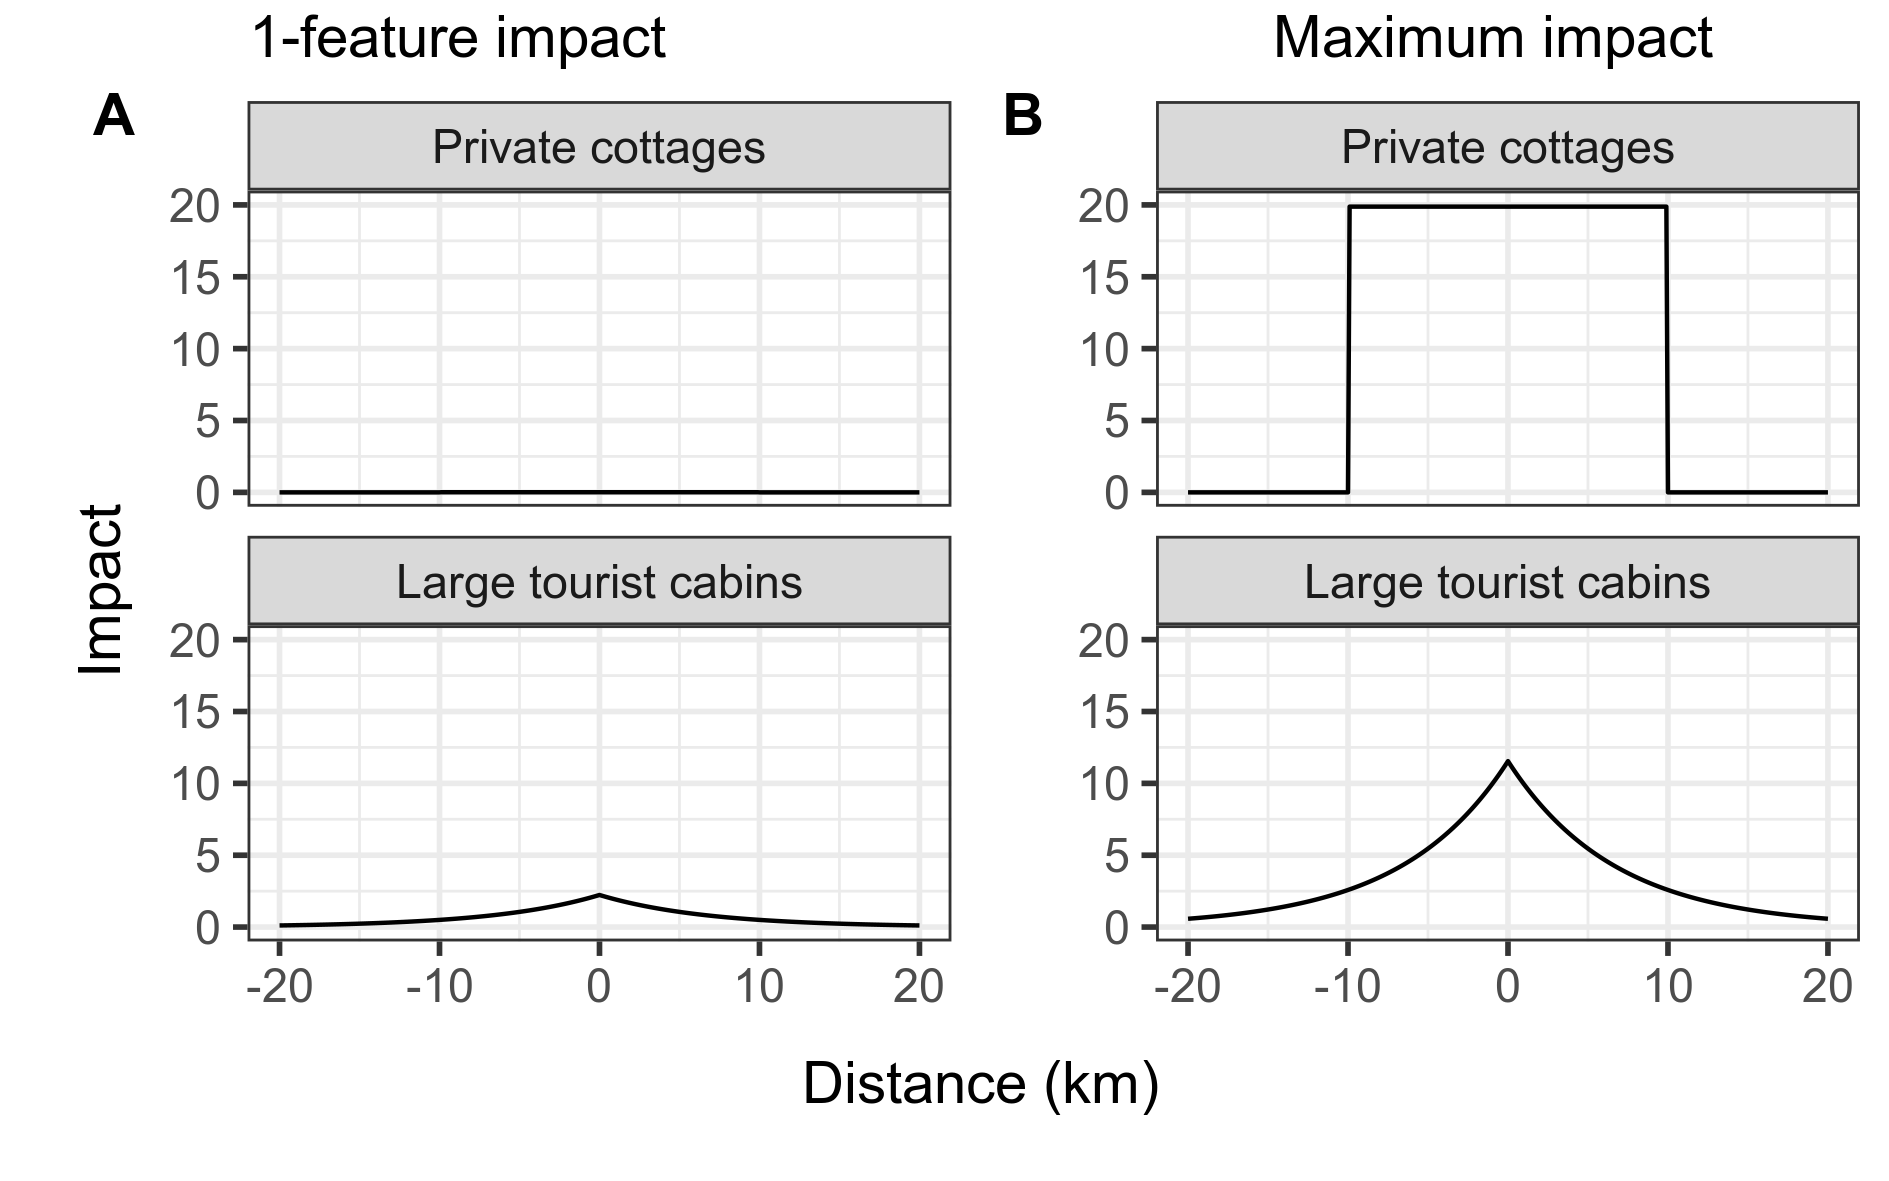
\includegraphics[width=1\textwidth,center]{figures/reindeer_zoi_impact_single_multiple_features.png}
\caption{\label{fig:impact_plot} Impact of private cottages and public cabins considering only 1 feature and the maximum number of each type of feature in the study area (2664 for cottages, 5 for cabins), given their respective influence functions and ZoI. The impact presented here is the multiplication between the magnitude of the impact (the model coefficients) and the cumulative influence variable (eq. \ref{eqn:HSFcuminf}). While the impact of only one private cottage is negligible, at their maximum densities the cumulative impact of private cottages might be higher than that of tourist cabins.}
\end{figure}

The estimated magnitude of the impact of a single private
cottage ($\beta_{cottage} = -0.00746$) was much smaller than that of a single tourist cabin
($\beta_{\text{private cabin}} = -2.233$; Table C3, Fig. \ref{fig:impact_plot}A), which is reasonable since the former are used by much less people than the latter. However, since
private cottages occur at much higher densities, in some areas their overall impact 
might be higher than that of tourist cabins. If we take the areas with the 
higher cumulative influence of infrastructure in Hardangervidda -- where the number of private cottages sum to 2664 
and the (exponentially weighted) number of tourist cabins sum to 5 -- the impact of 
private cottages agglomerates can be several times higher than that of tourist cabins
 (Fig. \ref{fig:impact_plot}B and 4). Following the HSF coefficient interpretation from \citealp{fieberg_how_2021}, considering that all other conditions are kept similar but each of these 
cumulative influence variables is changed by 1 standard deviation (1 SD = 491 for private cottages and
1 SD = 0.79 for tourist cabins), reindeer are nearly 38.9 times more likely to select an area with less private cottages and 5.8 times more likely
to select an area with less tourist cabins (Table C3, Appendix C).

When cumulative impacts of infrastructure are spatialized by multiplying the magnitude of the impacts to the cumulative influence measures (eq. \ref{eqn:HSFcuminf}), we see how the relative impact of private cottages and large tourist cabins change across space (Fig. \ref{fig:prediction_maps}). While the scaled impact value for private cottage goes to 1 in the areas with the highest cumulative influence of cottages, it hardly goes above 0.5 for tourist cabins. As a consequence the combined impact of multiple infrastructure, and given reindeer
avoided high densities of both infrastructure types at relatively large extents, 
areas of high habitat suitability for reindeer correspond to those in which the
cumulative influence of both infrastructure is low -- what matches the
locations used by reindeer, indicated through the GPS data (Fig. \ref{fig:prediction_maps}).

\begin{figure}[h]
\centering
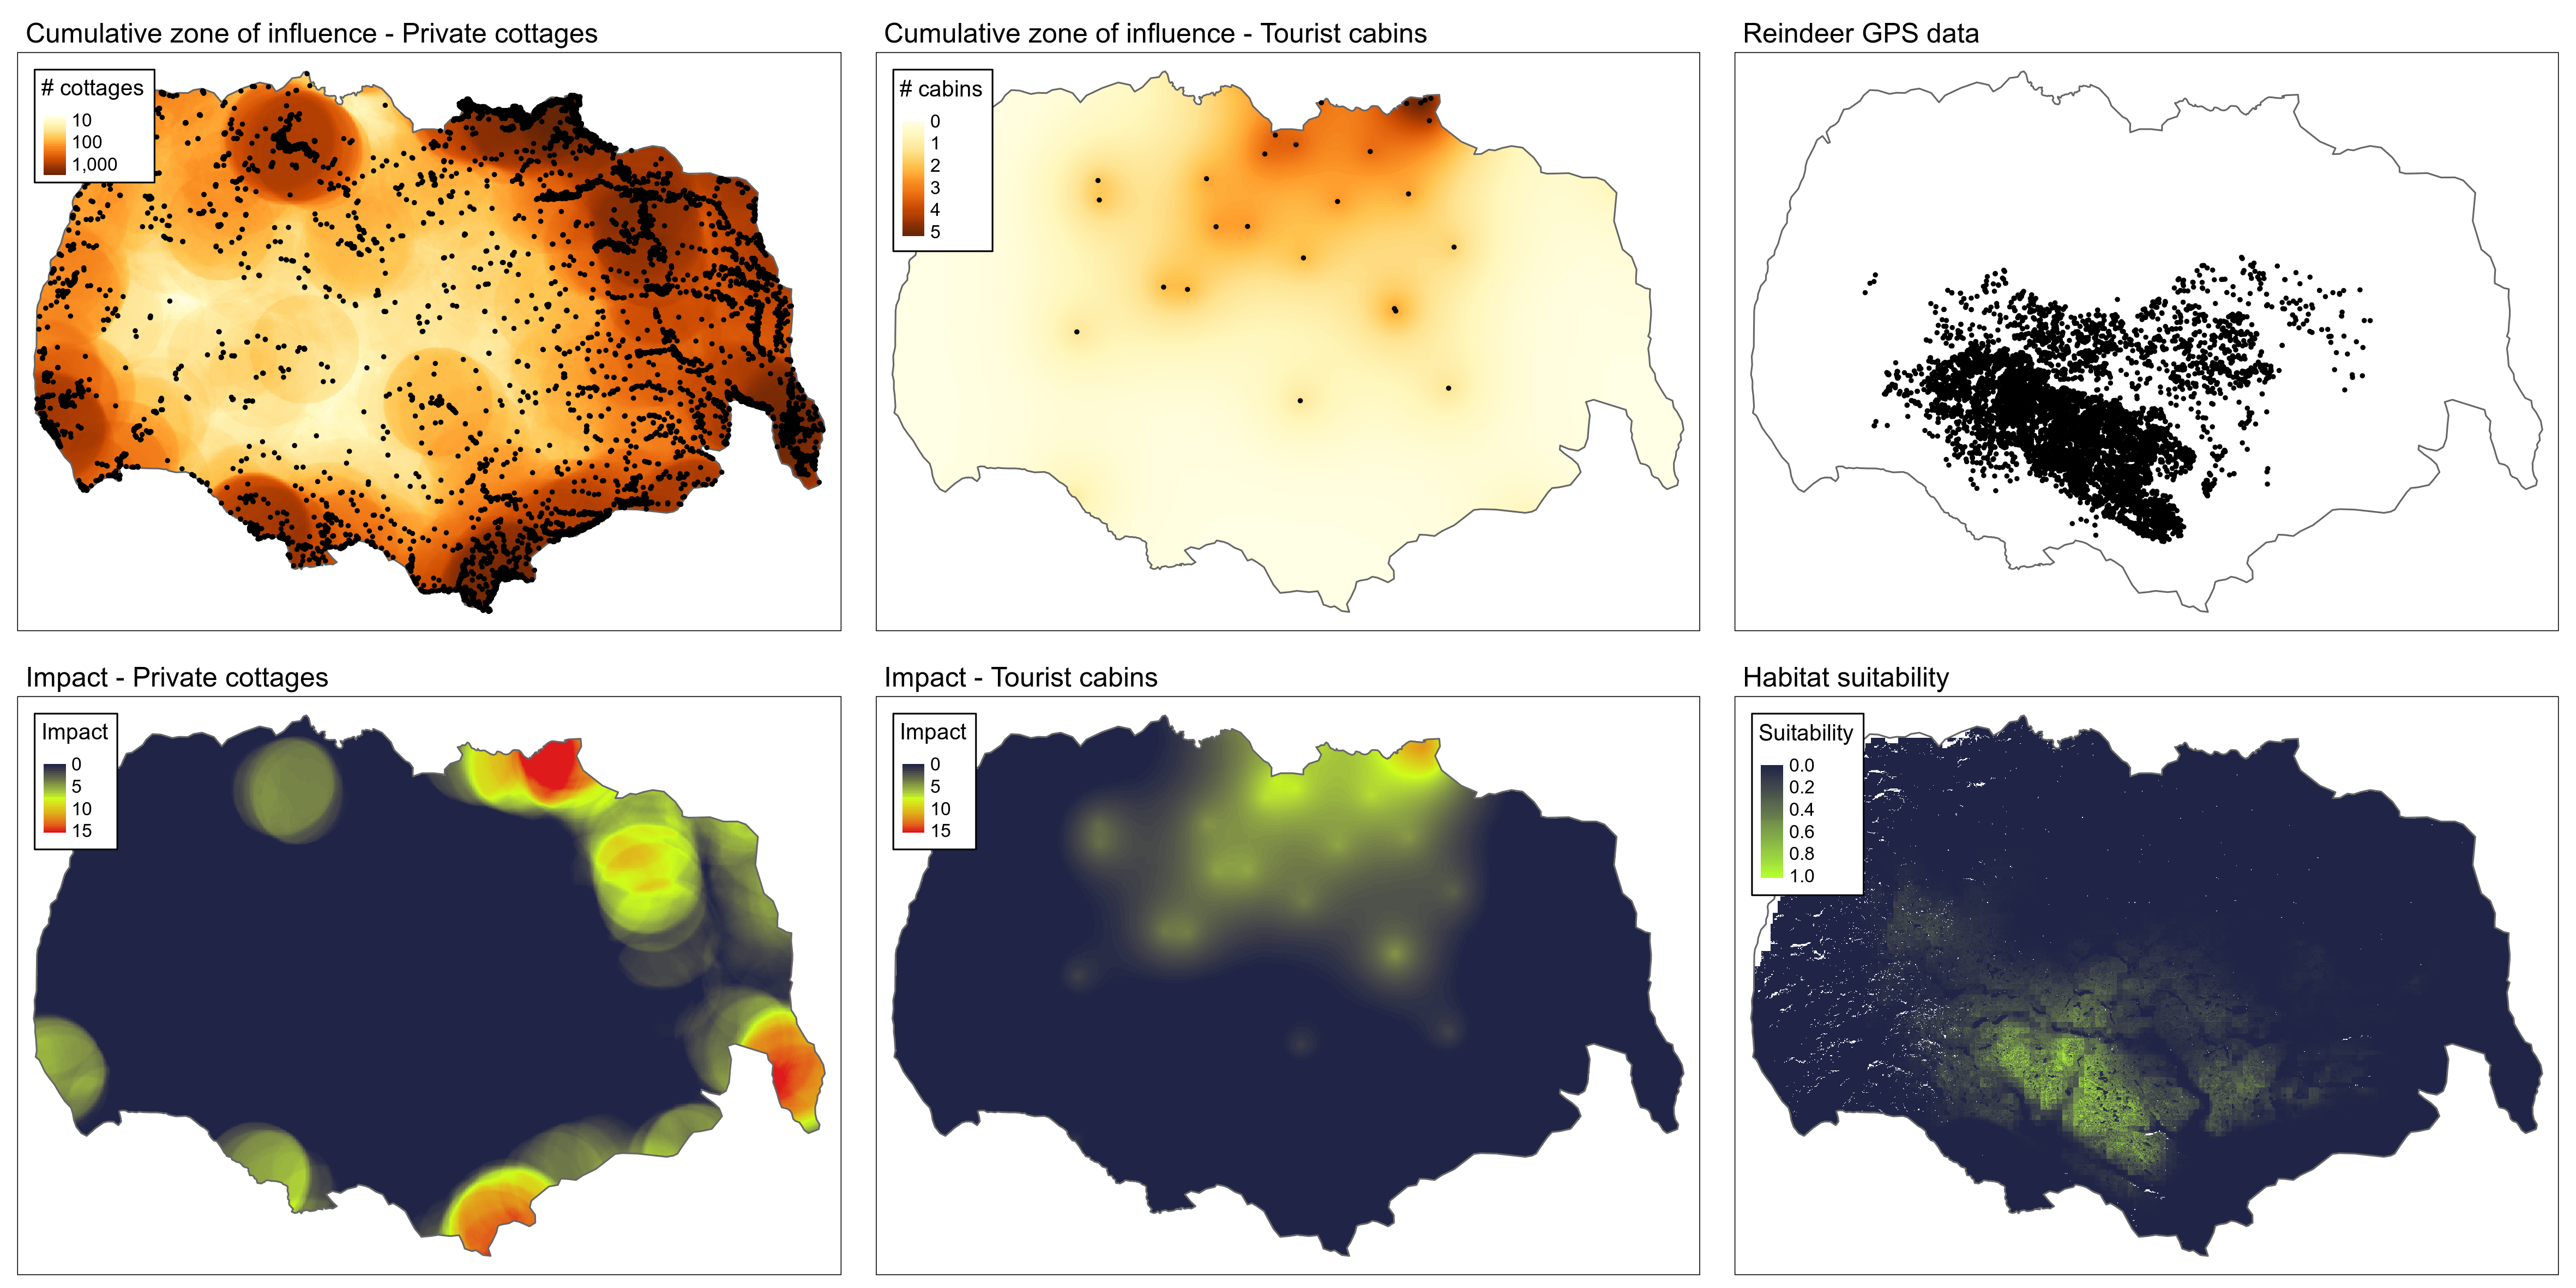
\includegraphics[width=1.3\textwidth,center]{figures/reindeer_results_prediction_maps.png}
\caption{\label{fig:prediction_maps} Maps of the most parsimonious cumulative influence variables (private cottages: threshold with 10km ZoI; tourist cabins: exponential decay with 20 km ZoI) and their estimated impacts on reindeer habitat selection for private cottages and large tourist cabins. These maps are showed alongside the reindeer GPS locations in the Hardengervidda wild reindeer area and the estimated reindeer habitat suitability. Notice that the most suitable areas correspond to areas with low cumulative influence of both private cottages and tourist cabins.}
\end{figure}

\section{Tools to assess cumulative impacts of infrastructure}

To ease the application of the cumulative effects assessment proposed here, we developed the \verb|oneimpact| R package. Based on raster maps with the location of infrastructure or any type of landscape variable (e.g. specific land cover or land use types), it allows the calculation of the influence from the nearest infrastructure feature ($\phi_{nearest}$ in eq. \ref{eqn:HSFnearest}) through the function \verb|calc_influence_nearest()| and the cumulative influence of multiple infrastructure ($\phi_{cum}$ in eq. \ref{eqn:HSFcuminf}) through the \verb|calc_influence_cumulative()| function. Both functions can be run using different filters or decay shapes (argument \verb|type|) -- exponential decay, linear (Bartlett or tent-shaped) decay, Gaussian (or half-normal) decay, threshold (or step) influence -- for multiple zones of influence (parameter \verb|zoi|), with the decay functions being parameterized on the ZoI. Besides those pre-defined decay functions, it also allows one to create user-defined filters (weight matrices) for cumulative effects estimation through the function \verb|create_filter()|.

Furthermore, the \verb|oneimpact| package allows the calculation of the influence measures on both R \citep{r_core_team_r_2020} and GRASS GIS \citep{grass_development_team_geographic_2017}. On the one hand, the implementation in R allows high accessibility to users, since R is the most used statistical tool by ecologists \citep{lai_evaluating_2019}. On the other hand, the package provides a direct link from R to the powerful algorithms of GRASS GIS, so the influence measure calculation might be performed for very large and fine-scale spatio-temporal datasets. An introduction to the essential functions to calculate the two influence measures is found in Appendices D (for R) and E (for GRASS GIS). The \verb|oneimpact| package is available in the Github repository: \url{github.com/NINAnor/oneimpact}.

\todo[inline]{Should we include a table with the functions and a short description?  Function name, description, type methods, input, output. Maybe in Appendix D.}

\section{Discussion}

There is an urge to evaluate, debate, and inform scientists, decision-makers, and the public 
in general about the past, current, and future effects of global infrastructure on biodiversity
\citep{laurance_conservation_2018}. Most of the decisions and regulations made for infrastructure
projects are performed with little knowledge about the multiple potential impacts on the ecosystems
where they are built and the species living therein. Even when environmental impact assessments are
well conducted, they hardly estimate the cumulative effects of those infrastructure with
pre-existing ones or with other development projects planned for the same region
\citep{laurance_roads_2017, krausman_cumulative_2011}. In great part, this happens 
because current approaches and tools still lack in their ability to incorporate 
cumulative impacts \citep[but see][for recent advances]{gillingham_integration_2016}. 
Building upon previous frameworks to understand cumulative impacts \citep{naugle_unifying_2011} 
and by adapting concepts and tools from the landscape ecology literature into the nearest 
and cumulative influence measures, here we gave a step further in developing a clear way to 
assess cumulative effects and impacts of infrastructure on biodiversity. 
The approach proposed here allows one to: (i) quantify the cumulative impact of 
multiple infrastructure of the same type; (ii) test whether there are cumulative 
impacts for each type of infrastructure, by comparing the influence of the nearest 
feature and the cumulative influence as predictors of biological responses, within 
ecological models; and (iii) estimate the zone of influence for multiple types of 
infrastructure. Here we depicted scenarios where each of the influence measures 
might converge or diverge, presented a case study to illustrate it, and offered tools 
to allow their application in ecological studies and environmental impact assessments.

The formulation of the influence of the nearest feature (eq. \ref{eqn:HSFnearest}) and the cumulative influence (eq. \ref{eqn:HSFcuminf}) as presented here makes it possible to compare whether there are cumulative effects of an infrastructure by comparing models with either of the influence measures, for instance through model fit estimates or variable selection (e.g. AIC or $R^2$; \citealt{jackson_are_2015, huais_multifit_2018}). It also raises the possibility of finding the ZoI (or scale of effect, \textit{sensu} \citealt{jackson_are_2015}) and the shape of decay of the influence with distance \citep[e.g. threshold or exponential decay, as in ][]{miguet_how_2017} only through model selection, without the necessity of performing complex parametrization of non-linear functions for multiple variables \citep{lee_estimating_2020}. In great part, this is feasible because the computation of these predictor variables might be performed before model fitting. 
Even though our current formulation (eq. \ref{eqn:HSFcuminf}) is maybe the simplest form of accounting for cumulative effects, more complex formats might be chosen, based on eq. \ref{eqn:HSFterm}, by changing the assumptions on the values of the effect sizes ($\beta's$) of each feature or the function shape of the decayment influence curves \citep{miguet_how_2017}. Yet, we believe out approach might be very useful in ecological studies.

To understand in which cases it might be more interesting to test for presence of cumulative effects, we used simulated scenarios with point infrastructure spread following different spatial point patterns and compared when the influence of the nearest feature and the cumulative influence of multiple features differ. For features that are regularly or randomly distributed, we found the two influence measures differ more strongly when the zone of influence increases. However, probably in most real situations infrastructure present some degree of clustering, for instance because they follow some pattern in the landscape (e.g. wind turbines built in mountain tops) or because they tend to be aggregated where there is already access through roads or waterways \citealp{barber_roads_2014}. In this case, the cumulative influence differs most from the influence of the nearest feature when the zone of influence is close to the size of the clusters (e.g. urban centers or wind parks), so using measures of infrastructure clustering might help indicate when it is expected to observe larger cumulative effects. In our simulated examples considered landscapes with point infrastructure because of the simplicity to represent them and place them following different patterns. We believe these simple cases might also provide insights on when $\phi_{nearest}$ and $\phi_{cum}$ are similar for other types of infrastructure, for instance linear infrastructure (e.g. roads, railways, and power lines) and higher dimensional landscape changes defined by polygons and areas (e.g. dams, mining or forestry areas, and deforestation sites). However, we recognize that those patterns can get more complex as these structures and spatial patterns extend over large distances and areas, and a further assessment of when these influence measures converge might be needed. In any case, as the ZoI is hardly known in advance for any system, we recommend a general approach of computing and using the two influence measures, to test if there is evidence of cumulative impacts in the different ecological systems and processes.

In our empirical demonstration with mountain reindeer in Norway, we found a strong support for the hypothesis of cumulative impacts of private cottages and tourist resorts on the reindeer habitat selection, with large ZoI (up to 20 km). Quantifying the impacts based on their magnitude and influence function allows us to compare the effects of different types of infrastructure. While the impact of a single cottage is much smaller than that of a single tourist cabins, it can be much higher in areas where many private cottages are aggregated (Fig. \ref{fig:impact_plot} and \ref{fig:prediction_maps}, Appendix C). It is important to notice that, if different influence functions are found to affect the ecological response under study, this has important consequences for the interpretation of the ZoI and the area affected by the infrastructure. For instance, while we found a constant influence of private cabins in a ZoI of 10 km, for tourist cabins we found an exponential decay of the influence of these infrastructure as one gets far from them, which means not all 20 km around resorts are affected equally. In a similar setup while evaluating the effects of landscape variables on the abundance of bird and insect species, \citet{miguet_how_2017} showed that the area affected by the landscape variable can increase by a factor of up to 5.7 when one uses a distance-weighted influence measure (as the exponential and Gaussian ones presented here), in comparison to a threshold-based landscape measure. 
We also found all models based on the influence of the nearest feature to perform much worse than the ones incorporating the cumulative influence of infrastructure. This includes the models based on the log-distance to the nearest feature, which is a common proxy for the effect of infrastructure and landscape variables in the ecological literature. This means that, researchers might have been ignoring 
the possibility of cumulative impacts, what might limit our overall understanding of the impacts of landscape change on biodiversity.

It is important to remark is that the extent of the study area and the scales or zones of influence to be tested must be carefully selected, especially in the context of cumulative impacts, when the interplay between multiple factors may produce complex setups. First, the effects of infrastructure on ecological processed might differ depending of the extent of the study area \citep{vistnes_matter_2008}. For instance, \cite{skarin_human_2014} showed that, depending of the temporal and spatial range of the study, the same type of infrastructure might vary in their effect to ecological variables, from no effect to positive or negative effects. As we show here, the spatial configuration of features and the ZoI might also affect our ability to detect if the impacts of infrastructure accumulate. Furthermore, the spatial pattern of features is also affected by the selection of extent of the landscape. As an example, if the biological response is measured and assessed in a study area that comprises 10 km around a wind farm, the distribution of wind turbines might look random or somehow aggregated. However, if the study area comprises a much bigger area and the biological response is expected to respond at larger extents, and the wind farm is only located in part of that, their distribution might appear very clumped. Second, the zones or scales of influence must be carefully selected. Depending on the biological response variable, the range of ZoI tested must encompass values much higher than the range size or even the average dispersal distance of an species \citep{jackson_what_2012,miguet_what_2016}. If the ZoI values are not properly defined, the ``true" scale at which the ecological process being measured is affected might not be selected, and the resulting estimated ZoI might be wrong and mislead decisions based on that \citep[e.g.][]{jackson_are_2015}.

Even though the examples given here focused on animal space use and habitat selection, the cumulative influence measure we presented is applicable over a wide range
of fields within ecology. First, the formulation in equation \ref{eqn:HSF} might be easily adapted to model other types of biological responses, such as population abundance REF[e.g.],
species richness REF[e.g.] or other measures of biological diversity and ecological processes REF[e.g.]. This might be achieved by setting the statistical models with the appropriate distributions, according to the the type of biological response variable (e.g., see Royle for models and model formulation), but the assumptions and use of the covariates and cumulative influence, as presented in eq. \ref{eqn:HSFterm}, \ref{eqn:HSFnearest}, and \ref{eqn:HSFcuminf} remain valid. Second, our approach might be used to calculate the nearest and cumulative influence measures either around sampling points (within discs or buffer areas; e.g. \citealt{huais_multifit_2018}) or calculated for the whole study area using multiple neighborhood sizes. The former might be particularly suited for ecological studies with a limited amount of sampling points, such as local landscape studies \citep[e.g.][]{muylaert_threshold_2016}. In the latter, the variables might be calculated for the whole study area and used to annotate data afterwards \citealp[e.g.][]{zeller_multi-level_2017}, allowing one to easily do that for thousands to millions of points, such as in movement ecology studies involving GPS data \citep[e.g.][]{tucker_moving_2018, davidson_ecological_2020} and species distribution modeling \citep{panzacchi_searching_2015}. In this case, the same spatial variables might also be useful for multiple projects and analyses in the same study area. The tools we provide here with the \verb|oneimpact| R package might help with these tasks.

\section{Conclusions}

There is an increasing need to include cumulative impacts on environmental regulation instruments, such as laws and legal instructions (?) for environmental assessment. However, even when they are present, bringing concepts and theoretical frameworks into concrete and objective analyses to estimate the impacts is often challenging and left to the responsibility of either the analysists or the regulators that review impact assessments \citep{johnson_regulating_2011,harris_grappling_2011}. Several studies point to the limitations of impact assessment only, mostly focused on the impacts of single projects, and advocate for a more systemic approach conducted at wider spatial extents and longer time periods \citep{laurance_conservation_2018,gillingham_integration_2016,krausman_cumulative_2011}. Approaches such as strategic impact assessments and regional land-use planning, for instance, might provide more comprehensive basis to estimate cumulative impacts and mitigate and plan on a longer term for future projects in a region. Our approach offers resources to ecologists, environmental agencies, and stakeholders dealing with impact assessment to build concrete estimates of cumulative impacts and their zone and area of influence. We hope this approach foments future discussion and research to make it easier and possible to include cumulative impacts in such regulation instruments.      
\section*{Authors’ contributions}

BBN, BVM, MP, MA, and AS conceived the idea. BBN, BVM and MP designed the methods, and analyzed and discussed the data. BBN, BVM, MP, TT, KL, and OS provided data. BBN and BVM wrote the first draft. All authors contributed with discussions and to the final version of the manuscript.

\section*{Acknowledgements}

P. Dodonov, M.H. Vancine for discussion around the implementation of the cumulative influence measures in R. NINA (or specific people) for the GPS data. E. Gurarie for his teaching on how to work on analyses and methodological approaches through R packages.

\section*{Conflicts of Interest}

The authors declare no conflicts of interest.

\section*{Data availability statement}

GPS data is archived in Movebank (www.movebank.org) and might be access upon request. All environmental data was retrieved from public repositories. The \verb|oneimpact| package is open and available at \url{github.com/NINAnor/oneimpact}, and all scripts used in the analyses are available in the Github repository \url{github.com/bniebuhr/cumulative_influence_paper} (to be made public upon the acceptance of the manuscript).

\section*{Supplementary Material}

Appendix A. Deriving the cumulative influence for line and polygon representations of infrastructure. \\
Appendix B. Simulating scenarios: comparing the the influence of the nearest feature with the cumulative influence of multiple features \\
Appendix C. Cumulative influence of infrastructure on reindeer space use: fitting habitat selection models \\
Appendix D. Getting started with \verb|oneimpact|. \\
Appendix E. Calculating cumulative influence in GRASS GIS using the \verb|oneimpact| package in R.

\bibliographystyle{besjournals}
\bibliography{cuminf_bib}

\end{document}
